\chapter{Câu hỏi ôn tập}
\hideall{
\setcounter{section}{0}
\begin{center}
	\textbf{\large BẢNG ĐÁP ÁN}
\end{center}
\section{Câu trắc nghiệm nhiều phương án lựa chọn}
\inputansbox{10}{ans/Y24-VN12-PH-C2-TN}
\section{Câu trắc nghiệm đúng sai}
\inputansbox[2]{2}{ans/Y24-VN12-PH-C2-TF}
\section{Câu trắc nghiệm trả lời ngắn}
\inputansbox[3]{6}{ans/Y24-VN12-PH-C2-TL}
}
\setcounter{section}{0}
\section{Câu trắc nghiệm nhiều phương án lựa chọn}
\textit{Thí sinh trả lời từ câu 1 đến câu 18. Mỗi câu thí sinh chọn một phương án}
\setcounter{ex}{0}
\Opensolutionfile{ans}[ans/Y24-VN12-PH-C2-TN]
% ===================================================================
\begin{ex}
	Khi nhiệt độ của một khối khí lý tưởng tăng ở áp suất không đổi, khối lượng riêng của khối khí sẽ như thế nào?
	\choice
	{\True Khối lượng riêng giảm}
	{Khối lượng riêng không thay đổi}
	{Khối lượng riêng có thể tăng hoặc giảm}
	{Khối lượng riêng tăng}
	\loigiai{}
\end{ex}
% ===================================================================
\begin{ex}
	Thiết bị nào sau đây không dùng để xác định nhiệt hoá hơi riêng của nước?
	\choice
	{Oát kế}
	{Cân điện tử}
	{Nhiệt lượng kế}
	{\True Nhiệt kế}
	\loigiai{}
\end{ex}
% ===================================================================
\begin{ex}
	Bơm căng săm xe đạp và vặn van thật chặt nhưng để lâu ngày vẫn bị xẹp lốp vì
	\choice
	{săm xe làm bằng cao su là chất đàn hồi, nên sau khi giãn ra thì tự động co lại làm cho săm để lâu ngày bị xẹp}
	{lúc bơm, không khí vào săm còn nóng, sau đó không khí nguội dần, co lại, làm săm xe bị xẹp}
	{\True giữa các phân tử cao su dùng làm săm có khoảng cách nên các phân tử không khí có thể thoát ra ngoài làm săm xẹp dần}
	{cao su dùng làm săm đẩy các phân tử không khí lại gần nhau nên săm bị xẹp}
	\loigiai{}
\end{ex}
% ===================================================================
\begin{ex}
	 Quần áo khô sau khi phơi dưới ánh nắng mặt trời. Hiện tượng này thể hiện?
	\choice
	{\True Sự bay hơi của nước}
	{Sự nóng chảy của nước}
	{Sự đông đặc của nước}
	{Sự ngưng tụ của nước}
	\loigiai{}
\end{ex}
% ===================================================================
\begin{ex}
Người ta ghi chép rằng tại cửa sông Amazon đã tìm thấy một thỏi vàng thiên nhiên có khối lượng $\SI{62.3}{\kilogram}$. Nếu khối lượng mol của vàng là $\SI{197}{\gram/\mole}$ thì số mol của thỏi vàng này gần giá trị nào nhất sau đây?	
	\choice
	{\SI{132}{\mole}}
	{\SI{457}{\mole}}
	{\SI{477}{\mole}}
	{\True \SI{316}{\mole}}
	\loigiai{}
\end{ex}
% ===================================================================
\begin{ex}
	Công thức nào sau đây là công thức tổng quát của định luật một nhiệt động lực học?
	\choice
	{$\Delta U=Q$}
	{\True $\Delta U=Q+A$}
	{$\Delta U=A$}
	{$A+Q=0$}
	\loigiai{}
\end{ex}
% ===================================================================
\begin{ex}
	Khi dùng các đèn cồn giống hệt nhau để đun các bình nước khác nhau trong cùng một khoảng thời gian, người ta thấy nhiệt độ trong các bình là khác nhau. Yếu tố nào sau đây làm cho nhiệt độ của nước ở trong các bình trở nên khác nhau khi ta đun nước?
	\choice
	{Thời gian đun}
	{Nhiệt lượng mà các bình nhận được}
	{\True Lượng chất lỏng chứa trong từng bình}
	{Loại chất lỏng chứa trong từng bình}
	\loigiai{}
\end{ex}
% ===================================================================
\begin{ex}
	Tính chất nào sau đây \textbf{không phải} của phân tử vật chất ở thể khí?
	\choice
	{chuyển động không ngừng}
	{chuyển động hỗn loạn}
	{chuyển động hỗn loạn và không ngừng}
	{\True chuyển động hỗn loạn xung quanh các vị trí cân bằng cố định}
	\loigiai{}
\end{ex}
% ===================================================================
\begin{ex}
	Một bọt khí nổi lên từ một đáy hồ nước. Khi đến mặt nước, nó có thể tích gấp 1,2 lần ban đầu. Coi nhiệt độ của bọt khí là không đổi. So với áp suất trên mặt hồ thì áp suất dưới đáy hồ
	\choice
	{lớn hơn 1,44 lần}
	{nhỏ hơn 1,2 lần}
	{nhỏ hơn 2,4 lần}
	{\True lớn hơn 1,2 lần}
	\loigiai{}
\end{ex}
% ===================================================================
\begin{ex}
	Gọi $p$ là áp suất, $V$ là thể tích, $R$ là hằng số khí lí tưởng, $k$ là hằng số Boltzmann và $T$ là nhiệt độ tuyệt đối. Số mol khí có trong một khối lượng chất khí cho trước được xác định bởi biểu thức
	\choice
	{$\dfrac{pR}{VT}$}
	{$\dfrac{pV}{kT}$}
	{\True $\dfrac{pV}{RT}$}
	{$pV$}
	\loigiai{}
\end{ex}
% ===================================================================
\begin{ex}
	Biết nhiệt nóng chảy riêng của nước đá là $\lambda=\SI{3.4E5}{\joule/\kilogram}$. Nhiệt lượng $Q$ cần cung cấp để làm nóng chảy hoàn toàn $\SI{100}{\gram}$ nước đá ở $\SI{0}{\celsius}$ bằng
	\choice
	{$\SI{340E5}{\joule}$}
	{$\SI{0.34E3}{\joule}$}
	{$\SI{34E7}{\joule}$}
	{\True $\SI{34E3}{\joule}$}
	\loigiai{}
\end{ex}
% ===================================================================
\begin{ex}
	Phát biểu nào sau đây về nội năng là không đúng?
	\choice
	{Nội năng là một dạng năng lượng}
	{Nội năng có thể chuyển hoá thành các dạng năng lượng khác}
	{\True Nội năng là nhiệt lượng}
	{Nội năng của một vật có thể tăng lên, giảm đi}
	\loigiai{}
\end{ex}
% ===================================================================
\begin{ex}
	Nhiệt độ mùa đông tại thành phố NewYork (Mĩ) là $\SI{23}{\degree F}$. Ứng với nhiệt Celsius, nhiệt độ đó là
	\choice
	{\SI{10}{\celsius}}
	{\SI{-10}{\celsius}}
	{\SI{5}{\celsius}}
	{\True \SI{-5}{\celsius}}
	\loigiai{}
\end{ex}
% ===================================================================
\begin{ex}
	Bảng bên dưới cho biết nhiệt độ nóng chảy và nhiệt độ sôi của bốn chất.
\begin{center}
		\begin{tabular}{|M{5cm}|M{5cm}|M{5cm}|}
		\hline 
		\thead{Chất} & \thead{Nhiệt độ nóng chảy $\left(\si{\celsius}\right)$} & \thead{Nhiệt độ sôi $\left(\si{\celsius}\right)$} \\
		\hline 1 & $-210$ & $-196$ \\
		\hline 2 & $-39$ & 357 \\
		\hline 3 & 30 & 2400 \\
		\hline 4 & 327 & 1749 \\
		\hline
	\end{tabular}
\end{center}
	\choice
	{Chất 1}
	{\True Chất 2}
	{Chất 3}
	{Chất 4}
	\loigiai{}
\end{ex}
% ===================================================================
\begin{ex}
	\immini{Một khối khí thực hiện các quá trình biến đổi trạng thái như hình bên. Ý nào sau đây là \textbf{không đúng}?
		\choice
		{\True AB là quá trình nén đẳng tích}
		{$\dfrac{V_{\mathrm{A}}}{T_{\mathrm{A}}}=\dfrac{V_{\mathrm{B}}}{T_{\mathrm{B}}}$}
		{CA là quá trình dãn nở đẳng nhiệt}
		{$p_{\mathrm{A}}V_{\mathrm{A}}=p_{\mathrm{C}}V_{\mathrm{C}}$}}
		{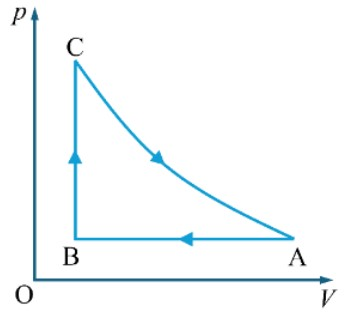
\includegraphics[scale=0.5]{../figs/Y24-VN12-PH-C2-BT-1}}
	\loigiai{}
\end{ex}
% ===================================================================
\begin{ex}
	Một nhiệt kế có phạm vi đo từ $\SI{263}{\kelvin}$ đến $\SI{1273}{\kelvin}$, dùng để đo nhiệt độ của các lò nung. Phạm vi đo của nhiệt kế này trong thang nhiệt độ Celsius là
	\choice
	{\SI{-12}{\celsius} và \SI{1000}{\celsius}}
	{\SI{-20}{\celsius} và \SI{1200}{\celsius}}
	{\SI{0}{\celsius} và \SI{273}{\celsius}}
	{\True \SI{-10}{\celsius} và \SI{1000}{\celsius}}
	\loigiai{}
\end{ex}
% ===================================================================
\begin{ex}
	Một học sinh sử dụng bộ thiết bị như hình a) bên dưới để so sánh năng lượng nhiệt cần thiết để làm nóng những khối vật liệu khác nhau. Mỗi khối có khối lượng bằng nhau và có nhiệt độ ban đầu là \SI{20}{\celsius}. Học sinh đó tiến hành đo thời gian cần thiết để nhiệt độ của mỗi khối vật liệu tăng lên thêm \SI{5}{\celsius}. Kết quả được biểu diễn trên hình b) bên dưới. Vật liệu nào có nhiệt dung riêng lớn nhất?
	\begin{center}
		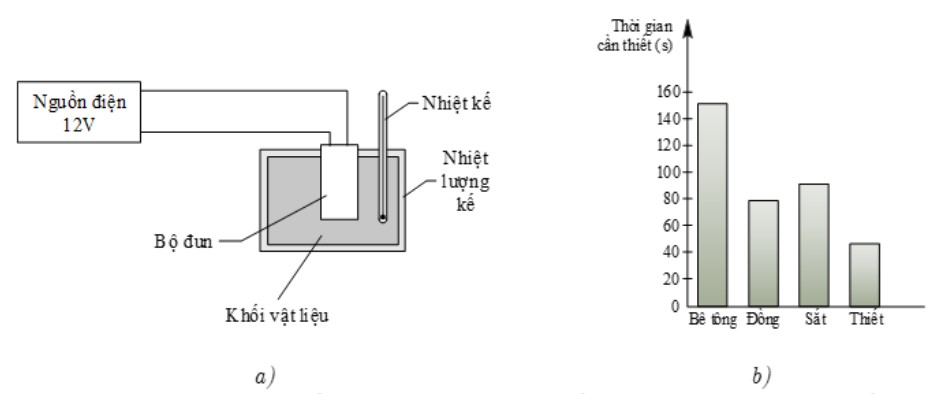
\includegraphics[scale=0.8]{../figs/Y24-VN12-PH-C2-BT-2}
	\end{center}
	\choice
	{\True Bê tông}
	{Thiếc}
	{Sắt}
	{Đồng}
	\loigiai{}
\end{ex}
% ===================================================================
\begin{ex}
	\immini{Trên đồ thị $\left(V, T\right)$ (xem hình vẽ bên) vẽ bốn đường đẳng áp của cùng một lượng khí. Đường ứng với áp suất thấp nhất là
		\choice
		{\True $p_4$}
		{$p_1$}
		{$p_3$}
		{$p_2$}}
		{\vspace{-0.75cm}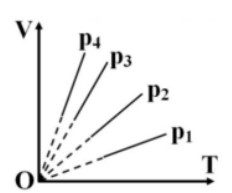
\includegraphics[scale=0.7]{../figs/Y24-VN12-PH-C2-BT-3}}
	\loigiai{}
\end{ex}
\Closesolutionfile{ans}
\section{Câu trắc nghiệm đúng sai}
\textit{Thí sinh trả lời từ câu 1 đến câu 4. Trong mỗi ý \textbf{a)}, \textbf{b}, \textbf{c)}, \textbf{d)} ở mỗi câu, thí sinh chọn đúng hoặc sai}
\setcounter{ex}{0}
\Opensolutionfile{ans}[ans/Y24-VN12-PH-C2-TF]
% ===================================================================
\begin{ex}
	\immini{Một nhóm học sinh tìm hiểu về mối liên hệ giữa áp suất và thể tích của một lượng khí xác định khi nhiệt độ được giữ không đổi. Họ đã thực hiện các nội dung sau: Chuẩn bị bộ thí nghiệm (hình bên) dịch chuyển từ từ pit tông để làm thay đổi thể tích của khí, đọc và ghi kết quả áp suất, thể tích theo số chỉ của dụng cụ đo kết quả như bảng bên}
	{\vspace{-0.75cm}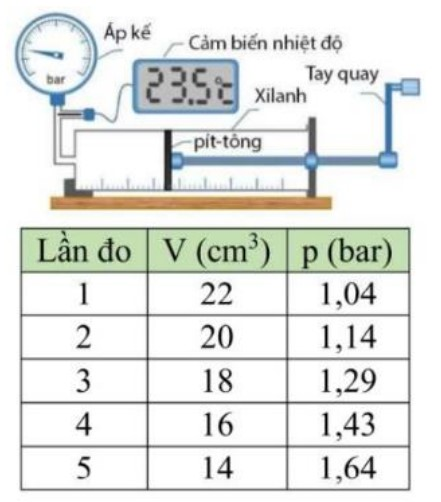
\includegraphics[scale=0.5]{../figs/Y24-VN12-PH-C2-BT-4}}
	\choiceTF[t]
	{Khi tiến hành thí nghiệm nhóm đã dịch chuyển từ từ pit tông để mục đích chính là giúp toàn thể các bạn trong nhóm có thời gian để nhìn rõ kết quả thay đổi các thông số của khí}
	{Bỏ qua sai số coi công thức liên hệ áp suất theo thể tích là $p=\dfrac{23}{V}$, $p$ đo bằng bar $\left(\SI{1}{bar}=\SI{E5}{\pascal}\right)$, $V$ đo bằng $\si{\centi\meter^3}$. Thể tích khí đã dùng trong thí nghiệm ở điều kiện tiêu chuẩn là 0,18 lít}
	{\True Số liệu thí nghiệm cho thấy áp suất tỉ lệ nghịch với thể tích của nó}
	{\True Thí nghiệm này đã kiểm chứng được định luật Boyle}
	\loigiai{}
\end{ex}
% ===================================================================
\begin{ex}
	\immini{Ngày 26 tháng 10 năm 2024 đã diễn ra lễ hội khinh khí cầu Tràng An - Cúc Phương năm 2024 tại Ninh Bình. Một khí cầu có thể tích $V=\SI{336}{\meter^3}$ và khối lượng vỏ $m=\SI{82}{\kilogram}$ được bơm không khí nóng tới áp suất bằng áp suất không khí bên ngoài. Biết không khí bên ngoài có nhiệt độ $\SI{30}{\celsius}$ và áp suất $\SI{1}{atm}$ (với $\SI{1}{atm}=\SI{101325}{\pascal}$); khối lượng mol của không khí ở điều kiện chuẩn là $\SI{29E-3}{\kilogram/\mole}$.}
	{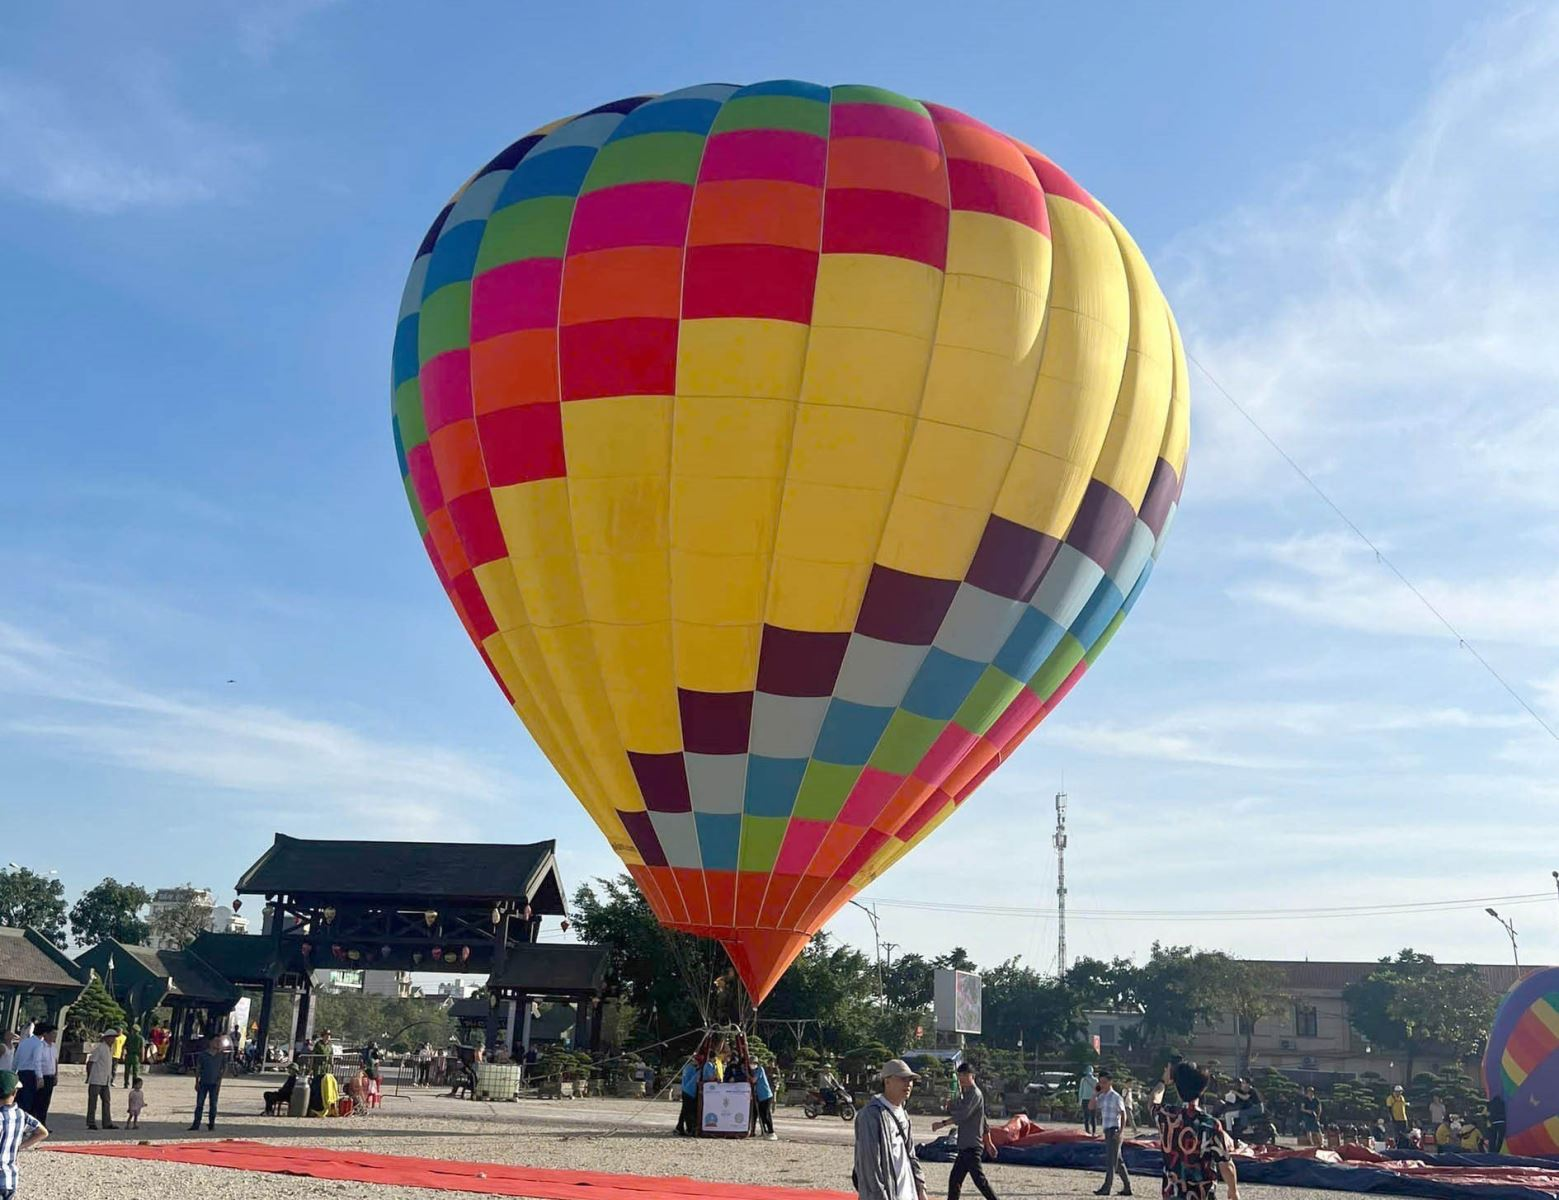
\includegraphics[scale=0.1]{../figs/Y24-VN12-PH-C2-BT-5}}
	\choiceTF[t]
	{\True Nhiệt độ của không khí bên ngoài khí cầu là $\SI{303}{\kelvin}$}
	{\True Khối lượng riêng của không khí ở nhiệt độ $\SI{30}{\celsius}$ và áp suất \SI{1}{atm} là $\SI{1.17}{\gram/\liter}$}
	{\True Cho rằng lực của gió không đáng kể, lực chính đẩy khí cầu bay lên là lực Archimedes tác dụng vào khí cầu}
	{Cho rằng lực của gió không đáng kể để khí cầu bắt đầu bay lên thì nhiệt độ không khí nóng bên trong khí cầu là $\SI{368}{\kelvin}$}
	\loigiai{\begin{itemchoice}
			\itemch Đúng. $T=t+273=\SI{303}{\kelvin}$.
			\itemch Đúng. $\dfrac{p_0}{D_0T_0}=\dfrac{R}{M}\Leftrightarrow \dfrac{101325}{D_0\left(30+273\right)}=\dfrac{8,31}{\SI{29E-3}{}}\Rightarrow D_0\approx\SI{1.167}{\kilogram/\meter^3}=\SI{1.17}{\gram/\liter}$.
			\itemch Đúng. 
			\itemch Sai. \\
			$F_A=P\Rightarrow D_0gV=mg+DgV
			\Rightarrow 1,167\cdot336=82+D\cdot336\Rightarrow D\approx\SI{0.923}{\kilogram/\meter^3}$\\
			$\dfrac{p}{DT}=\dfrac{R}{M}\Rightarrow\dfrac{101325}{0,923\cdot T}=\dfrac{8,31}{\SI{29E-3}{}}\Rightarrow T\approx\SI{383}{\kelvin}$.
	\end{itemchoice}}
\end{ex}
% ===================================================================
\begin{ex}
\immini{	Một nhóm học sinh tìm hiểu về sự truyền nhiệt. Họ có các dụng cụ và cách tiến hành như sau: \\
	\textbf{Dụng cụ}\\
	\begin{itemize}
		\item Cốc nhôm đựng $\SI{200}{\milli\liter}$ nước ở nhiệt độ \SI{30}{\celsius} (1).
		\item Bình cách nhiệt đựng \SI{500}{\milli\liter} nước ở nhiệt độ \SI{60}{\celsius} (2).
		\item Hai nhiệt kế (3).
	\end{itemize}
	\textbf{Tiến hành}
	}
	{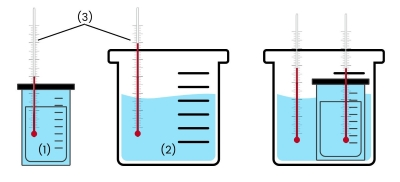
\includegraphics[scale=0.6]{../figs/Y24-VN12-PH-C2-BT-6}}
	\vspace{0.5cm}
\begin{itemize}
	\item Đặt cốc nhôm vào trong lòng bình cách nhiệt như hình vẽ và quan sát số chỉ nhiệt kế để tìm hiểu về sự truyền nhiệt của chúng.
\end{itemize}
	\choiceTF[t]
	{\True Nhiệt độ nước ở bình (2) giảm dần chứng tỏ nó thực hiện truyền nhiệt lượng}
	{\True Nhiệt độ nước trong cốc nhôm (1) tăng dần chứng tỏ nước trong cốc (1) được nhận nhiệt lượng}
	{Sau một thời gian cả hai nhiệt kế chỉ giá trị không đổi và bằng nhau chứng tỏ sự truyền nhiệt năng đã dừng lại khi nước trong hai bình tràn vào nhau có thể tích bằng nhau}
	{Thí nghiệm này có thể kiểm chứng cho kết luận: nhiệt năng truyền từ vật có khối lượng lớn hơn sang vật có khối lượng nhỏ hơn}
	\loigiai{}
\end{ex}
% ===================================================================
\begin{ex}
	\immini{Một học sinh tiến hành đun một khối nước đá đựng trong nhiệt lượng kế từ \SI{0}{\celsius} đến khi tan chảy hết thành nước và hóa hơi ở \SI{100}{\celsius}. Hình bên là đồ thị biểu diễn sự phụ thuộc của nhiệt lượng mà khối nước đá nhận được từ lúc đun đến lúc bay hơi và sự thay đổi nhiệt độ của nó. Lấy nhiệt nóng chảy riêng của nước đá là \SI{3.3E5}{\joule/\kilogram} và nhiệt dung riêng của nước đá là \SI{4200}{\joule/\kilogram},
		nhiệt hóa hơi riêng của nước là \SI{2.3E6}{\joule/\kilogram}, bỏ qua nhiệt dung của nhiệt lượng kế.}
		{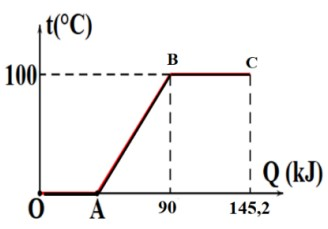
\includegraphics[scale=0.8]{../figs/Y24-VN12-PH-C2-BT-7}}
	\choiceTF[t]
	{\True Tại điểm B trên đồ thị, nước bắt đầu xảy ra sự sôi}
	{\True Trong đoạn BC trên đồ thị, khối nước nhận nhiệt lượng để thực hiện quá trình hóa hơi}
	{\True Tại điểm C lượng nước còn lại là \SI{96}{\gram}}
	{Nếu tiến hành đun đến khi lượng nước bay hơi hết cần cung cấp nhiệt lượng tổng cộng là \SI{325}{\kilo\joule}}
	\loigiai{\begin{itemchoice}
			\itemch Đúng. 
			\itemch Đúng. 
			\itemch Đúng. $Q_B=m\left(\lambda+c\Delta t\right)\Leftrightarrow 90\cdot10^3=m\left(\SI{3.3E5}{}+4200\cdot100\right)\Rightarrow m=\SI{0.12}{\kilogram}$.\\
			$m_{\mathrm{BC}}=\dfrac{Q_C-Q_B}{L}=\SI{0.024}{\kilogram}$.\\
			Tại điểm C lượng nước còn lại là $m-m_{\mathrm{BC}}=0,12-0,024=\SI{0.096}{\kilogram}=\SI{96}{\gram}$.
			\itemch Sai. $Q_B+mL=90\cdot10^3+0,12\cdot2,3\cdot10^6=\SI{366}{\kilo\joule}$.
	\end{itemchoice}}
\end{ex}
\Closesolutionfile{ans}
\section{Câu trắc nghiệm trả lời ngắn} \textit{Thí sinh trả lời từ câu 1 đến câu 6}
\setcounter{ex}{0}
\Opensolutionfile{ans}[ans/Y24-VN12-PH-C2-TL]
% ===============================================================
\begin{ex}
	Một săm xe máy được bơm không khí ở \SI{27}{\celsius} tới áp suất \SI{2}{atm}. Săm chỉ có thể chịu được áp suất tối đa bằng \SI{3.0}{atm}. Bỏ qua sự nở nhiệt của săm. Nhiệt độ của không khí trong săm có thể có giá trị lớn nhất bằng bao nhiêu $\si{\celsius}$ để săm không bị nổ? (làm tròn kết quả đến chữ số hàng đơn vị).
	\shortans[oly]{177}
	\loigiai{
		$\dfrac{p}{T}=const\Rightarrow \dfrac{2}{27+273}=\dfrac{3}{T}\Rightarrow T=\SI{450}{\kelvin}\approx\SI{177}{\celsius}$.
	}
\end{ex}
% ===============================================================
\begin{ex}
Một bình đựng \SI{2.5}{\gram} khí helium có thể tích 5 lít và nhiệt độ ở \SI{27}{\celsius}. Áp suất khí trong bình là $\xsi{x\cdot10^5}{\newton/\meter^2}$. Giá trị của $x$ bằng bao nhiêu? (kết quả lấy 1 chữ số sau dấu phẩy thập phân).	
	\shortans[oly]{3,1}
	\loigiai{
	$pV=\dfrac{m}{M}RT\Rightarrow p\approx\SI{3.1e5}{\pascal}$.	
	}
\end{ex}
% ===============================================================
\begin{ex}
	\immini{Khi thở ra, dung tích của phổi là $\SI{2,400}{\liter}$ và áp suất của không khí trong phổi là \SI{101,70E3}{\pascal}. Cho biết khi hít vào, áp suất này trở thành \SI{101,12E3}{\pascal}. Dung tích của phổi khi hít vào là bao nhiêu lít? (kết quả lấy 2 chữ số sau dấu phẩy thập phân).}
	{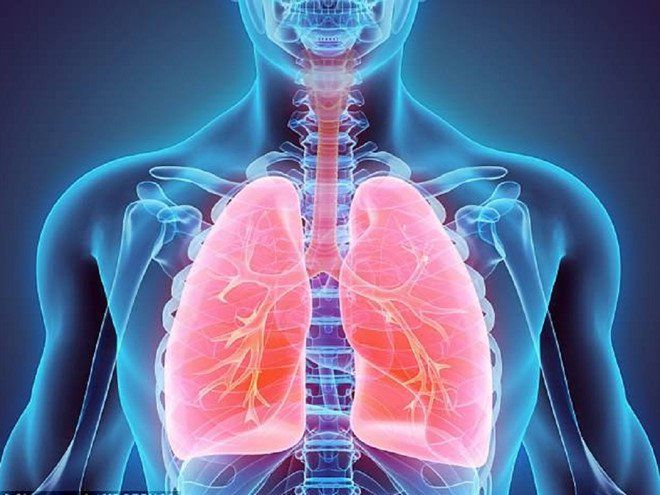
\includegraphics[scale=0.1]{../figs/Y24-VN12-PH-C2-BT-8}}
	\shortans[oly]{2,41}
	\loigiai{
		$pV=const\Rightarrow 2,4\cdot101,7\cdot10^3=101,12\cdot10^3\cdot V\Rightarrow V\approx\SI{2.41}{\liter}$.
	}
\end{ex}
% ===============================================================
\begin{ex}
	Một lượng khí nhận một nhiệt lượng \SI{25.4}{\kilo\joule} do được đun nóng, khí giãn ra và thực hiện một công \SI{21.2}{\kilo\joule} ra môi trường xung quanh. Nội năng của khối khí này đã biến thiên một lượng bao nhiêu kilôjun (kJ)?
	\shortans[oly]{4,2}
	\loigiai{
		$\Delta U=Q+A=25,4-21,2=\SI{4.2}{\kilo\joule}$.
	}
\end{ex}
% ===============================================================
\begin{ex}
	\immini{Chuông lặn là một thiết bị chìm dưới nước để nghiên cứu các điều kiện trong nước, cũng có thể được sử dụng làm thiết bị lặn để sửa chữa các bộ phận dưới nước của trụ cầu và các công trình xây dựng khác. Một chuông lặn cao \SI{2}{\meter} được thả chìm theo phương thẳng đứng từ mặt nước xuống đáy hồ nước sâu \SI{8}{\meter} (hình vẽ). Giả sử nhiệt độ của khối khí (coi là khí lí tưởng) kèm theo trong chuông không đổi, áp suất khí quyển $p_0=\SI{E5}{\pascal}$, khối lượng riêng của nước là $\rho=\SI{E3}{\kilogram/\meter^3}$ và lấy $g=\SI{10}{\meter/\second^2}$. Độ cao $h$ của mực nước trong chuông bằng bao nhiêu mét? Kết quả lấy đến hai chữ số sau dấu phẩy thập phân.}
	{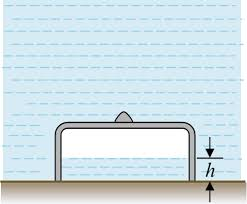
\includegraphics[scale=0.4]{../figs/Y24-VN12-PH-C2-BT-9}}
	\shortans[oly]{0,83}
	\loigiai{
		\begin{center}
			\begin{tabular}{|M{8cm}|M{8cm}|}
				\hline
				$p$ & $V$\\
				\hline
				$p_0=\SI{E5}{\pascal}$ & $S\cdot 2$\\
				\hline
				$p_0+Dg\left(8-h\right)=10^5+10^3\cdot10\left(8-h\right)$ & $S\cdot\left(2-h\right)$\\
				\hline
			\end{tabular}
		\end{center}
		$pV=const\Rightarrow 10^5\cdot S\cdot2=\left[10^5+10^3\cdot 10\cdot\left(8-h\right)\right]\cdot S\cdot\left(2-h\right)\Rightarrow h\approx\SI{0.83}{\meter}$.
	}
\end{ex}
% ===============================================================
\begin{ex}
	\immini{Vào mùa hè, người Hà Nội thường có thói quen thưởng thức trà đá trong các quán vỉa hè. Để có một cốc trà đá chất lượng, người chủ quán rót khoảng $\SI{0.250}{\kilogram}$ trà nóng ở \SI{80.0}{\celsius} vào cốc, sau đó cho tiếp $\xsi{m}{\kilogram}$ nước đá \SI{0}{\celsius}. Cuối cùng được cốc trà đá ở nhiệt độ phù hợp nhất là \SI{10.0}{\celsius} (hệ vừa đạt đến trạng thái cân bằng nhiệt). Biết phần nhiệt lượng mà hệ (nước và nước đá) nhận thêm của môi trường xung quanh bằng \SI{10}{\percent} nhiệt lượng mà các cục nước đá nhận để làm tăng nội năng của chúng. Nhiệt dung riêng của nước là \SI{4.20}{\kilo\joule/\kilogram\cdot\kelvin}; nhiệt nóng chảy của nước đá là \SI{3.33E5}{\joule/\kilogram}. Tính $m$ theo đơn vị $\si{\kilogram}$. Lấy 2 chữ số ở phần thập phân.}
	{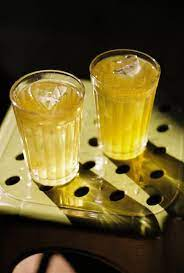
\includegraphics[scale=0.4]{../figs/Y24-VN12-PH-C2-BT-10}}
	\shortans[oly]{0,22}
	\loigiai{
		Nhiệt lượng nước tỏa ra + Nhiệt lượng môi trường cung cấp = Nhiệt lượng nước đá nhận vào để nóng chảy và tăng nhiệt độ.\\
		$Q_n+0,1\left(Q_{nc}+Q_{\text{đ}}\right)=Q_{nc}+Q_{\text{đ}}\Rightarrow Q_n=0,9\left(Q_{nc}+Q_{\text{đ}}\right)\Rightarrow m_nc_n\Delta t=0,9m\left(\lambda+c_n t_{cb}\right)$\\
		$\Leftrightarrow 0,25\cdot4,2\cdot10^3\cdot\left(80-10\right)=0,9m\left(3,33\cdot10^5+4,2\cdot10^3\cdot10\right)\Rightarrow m\approx\SI{0.22}{\kilogram}$.
	}
\end{ex}
\Closesolutionfile{ans}
\begin{center}
	\textbf{-- HẾT --}
\end{center}